
\newpage
\begin{tikzpicture}[remember picture, overlay]
	\node [inner sep=0pt, minimum width=\paperwidth, minimum height=\paperheight,opacity=.3] at (current page.center) {\includegraphics[width=\paperwidth,height=\paperheight,angle=0]{paper23}};
	\node [inner sep=0pt, minimum width=.9\paperwidth, minimum height=\paperheight,opacity=1,xshift=.25\paperwidth,text width=.5\linewidth,yshift=0.\paperheight] at (current page.center) {\includegraphics[width=.4\paperwidth,angle=0]{escalera1}};
\end{tikzpicture}
MUCHAS ESCALERAS MODERNAS SE FABRICAN DE TRAMOS RECTOS, PERO LAS MÁS BONITAS SON LAS QUE SE DESPLIEGAN DESDE ESPIRALES. ENTRE ELLAS, OÍ HABLAR EN EL BARRIO, HAY UNAS QUE 
\vspace{.5\paperheight}


SE DESTACAN POR SUS MATERIALES Y ACABADO MARAVILLOSOS. SE ENCUENTRAN EN EL MISTERIOSO CASTILLO DE VILLA DEL PARQUE.

\newpage
\begin{tikzpicture}[remember picture, overlay]
	\node [inner sep=0pt, minimum width=\paperwidth, minimum height=\paperheight,opacity=.3] at (current page.center) {\includegraphics[width=\paperwidth,height=\paperheight,angle=0]{paper22}};
	\node [inner sep=0pt, minimum width=.9\paperwidth, minimum height=\paperheight,opacity=1,xshift=.29\paperwidth,text width=.5\linewidth,yshift=0.\paperheight] at (current page.center) {\includegraphics[width=.4\paperwidth,angle=0]{castillo1}};
\end{tikzpicture}
SEGURAMENTE HABRÁN PASADO POR 

DELANTE DEL EDIFICIO QUE LLAMAN

TAMBIÉN ´´PALACIO DEL LOS BICHOS´´,

NOMBRE MUY PROMETEDOR PARA NOSOTROS

LOS FELINOS. 

TODO COMENZÓ EN UNA VISITA QUE HABÍA 

REALIZADO DONDE CONOCÍ A DOS AMIGAS, 

DORA Y MORA, DOS GATAS GRISES QUE

VIVEN POR VILLA DEL PARQUE. 
SON ELLAS 

MUY TRANQUILAS Y 
CARIÑOSAS  CON 

TANIA
Y CHALY, 
LOS HUMANOS A CARGO. 

TIENEN TODO OTRO ESTILO, NO 
DISFRUTAN 

DE DAR ZARPAZOS NI 
MORDIDAS.

EXTRAÑO.

\newpage
\begin{tikzpicture}[remember picture, overlay]
	\node [inner sep=0pt, minimum width=\paperwidth, minimum height=\paperheight,opacity=.3] at (current page.center) {\includegraphics[width=\paperwidth,height=\paperheight,angle=0]{paper22}};
	\node [inner sep=0pt, minimum width=.9\paperwidth, minimum height=\paperheight,opacity=1,xshift=.29\paperwidth,text width=.5\linewidth,yshift=0.\paperheight] at (current page.center) {\includegraphics[width=.4\paperwidth,angle=0]{dora1}};
\end{tikzpicture}

BIENVENIDO, OTTOKO -ME HABÍA DICHO DORA- YO SOY  DORA Y MI HERMANA SE LLAMA MORA.  ES UN

PLACER CONOCERTE. 

NOSOTRAS NO SOMOS DE SALIR MUCHO, PERO 

NOS GUSTA RECIBIR VISITAS Y LEER 

HISTORIAS, EN OCASIONES DE ESAS 

QUE DAN MIEDO.

- NO CONOZCO MUCHO DE ESAS HISTORIAS.

AUNQUE VI ALGUNAS EN LA BIBLIOTECA 

DE MI PADRE, HABÍA UNOS ´'CUENTOS DE 

EDGAR ALLAN POE´´ CON DIBUJOS ESPELUZNANTES.

Y TAMBIÉN OTRAS DE H.P. LOVECRAFT$\ldots$ 


\newpage
\begin{tikzpicture}[remember picture, overlay]
	\node [inner sep=0pt, minimum width=\paperwidth, minimum height=\paperheight,opacity=.3] at (current page.center) {\includegraphics[width=\paperwidth,height=\paperheight,angle=0]{paper22}};
\end{tikzpicture}
- BUENO, PERO ESTA HISTORIA QUE TE VOY A CONTAR PUEDE QUE DÉ MÁS MIEDO PUES SUCEDIÓ CERCA DE NUESTRAS CASAS.

HACE MUCHO TIEMPO, VILLA DEL PARQUE ERAN UNAS POCAS CASAS AL LADO DE LA ESTACIÓN DE TREN, LA IGLESIA Y VARIAS GRANJAS. 

--¡TENÍAN GALLINAS EN LA GRANJAS?, PREGUNTÉ ATENTO.

ESO NO TIENE NINGUNA IMPORTANCIA, RESPONDIÓ DORA Y CONTINUÓ:

UN HOMBRE VIUDO VINO A INSTALARSE JUNTO A SU HIJA ALEJÁNDOSE DEL CENTRO DE LA CIUDAD PUES LES DESPERTABA RECUERDOS TRISTES. PARECE QUE HABÍA HECHO UNA GRAN FORTUNA COMO  COMPOSITOR Y PIANISTA DE LA GRAN MÚSICA.

--ESO NO PARECE DAR MUCHO MIEDO, COMENTÉ CON ACIERTO.

--¡HAY QUE SER PACIENTE!, INDICÓ MORA, Y DEJÓ QUE SU HERMANA PROSIGUIERA:

TENÍA GUSTOS EXCÉNTRICOS, Y QUISO CONSTRUIR UN CASTILLO QUE 

\newpage
\begin{tikzpicture}[remember picture, overlay]
	\node [inner sep=0pt, minimum width=\paperwidth, minimum height=\paperheight,opacity=.3] at (current page.center) {\includegraphics[width=\paperwidth,height=\paperheight,angle=0]{paper22}};
	\node [inner sep=0pt, minimum width=.9\paperwidth, minimum height=\paperheight,opacity=1,xshift=.29\paperwidth,text width=.5\linewidth,yshift=0.\paperheight,xshift=-.65\textwidth] at (current page.center) {\includegraphics[width=.4\paperwidth,angle=0]{gargola1}};
	
	\node [inner sep=0pt, minimum width=.9\paperwidth, minimum height=\paperheight,opacity=1,text width=.74\linewidth,yshift=0.\paperheight,xshift=.15\textwidth] at (current page.center) {TUVIERA LOS ENCANTOS DE TIEMPOS ANTIGUOS CON LAS COMODIDADES DE LA MODERNIDAD. TENDRÍA SEIS PISOS PERO CADA UNO DE ELLOS DE EXAGERADA ALTURA, SERÍA LA CONSTRUCCIÓN  MÁS ELEVADA DEL BARRIO. 
		
		SE FABRICARON ESPECIALMENTE MUCHOS $~~~~~$ACCESORIOS Y ADORNOS MUY RAROS. IMITANDO $~~~~~~$ALGUNAS VIEJAS IGLESIAS EUROPEAS, EN $~~~~$LA FACHADA DE LOS PISOS ELEVADOS Y EN LA TORRE DE LA CÚPULA SE COLOCARON GÁRGOLAS DE SEMBLANTES AMENAZANTES.
		
		LAS GÁRGOLAS CUMPLÍAN LA FUNCIÓN DE CONDUCIR EL AGUA DE LLUVIA PARA QUE NO SE DAÑARAN LOS EDIFICIOS, PERO TAMBIÉN SIMBÓLICAMENTE LOS PROTEGÍA CONTRA LOS MALOS ESPÍRITUS.};
	
\end{tikzpicture}


\newpage
\begin{tikzpicture}[remember picture, overlay]
	\node [inner sep=0pt, minimum width=\paperwidth, minimum height=\paperheight,opacity=.3] at (current page.center) {\includegraphics[width=\paperwidth,height=\paperheight,angle=0]{paper20}};
	\node [inner sep=0pt, minimum width=.9\paperwidth, minimum height=\paperheight,opacity=1,text width=.5\linewidth,yshift=-.2\paperheight,xshift=.32\textwidth] at (current page.center) {\includegraphics[width=.4\paperwidth,angle=0]{ottoko_escucha}};
	
	
\end{tikzpicture}
AUNQUE SABÍA QUE ERAN DE PIEDRA, ME IMAGINÉ CAZANDO A ESAS HORRIBLES GÁRGOLAS. O MÁS BIEN HUYENDO DE ELLAS, DADO MI MODERADO TAMAÑO. EN TODO CASO, SERÍA UNA AGITADA TAREA ENCONTRAR GÁRGOLAS VIVIENTES. PERO DORA CONTINUÓ:

´´UNA CANTIDAD DE DETALLES TAMBIÉN SE TRABAJARON EN EL INTERIOR DEL CASTILLO. EMPEZANDO POR LAS ESCALERAS DE MÁRMOL BLANCO DISEÑADAS SEGÚN AMPLIAS ESPIRALES$\ldots$´´ 

ESE MATERIAL ES RESBALADIZO Y SI ES

BLANCO HARÍA MUY VISIBLE A CUALQUIER

GATO NEGRO, PENSÉ DISCRETAMENTE. 

DORA SIGUIÓ DESCRIBIENDO BALCONES,

SALAS,  CORTINAS Y MOBILIARIOS, TODO 

DE MUY CUESTIONABLE  INTERÉS FELINO.

-¿Y CUANDO APARECE LA HISTORIA DE MIEDO?

-¡OH!, ¡PERO QUE IMPACIENTE MININO AZABACHE!  DE ACUERDO, IRÉ AL GRANO.

´´PASARON AÑOS Y LA CASA IBA A INAUGURARSE EL DÍA DEL CASAMIENTO DE LA HIJA DEL DUEÑO, AMELIA. HABÍA ESTUDIADO EN UNA GRAN ESCUELA DE PARIS, COSA MUY RARA PARA LA ÉPOCA QUE UNA JOVEN REALIZARA ESTUDIOS UNIVERSITARIAS, PERO ASÍ COMO CONOCEN A MARIE CURIE, HUBO OTRAS.

ELLA VIVIÓ EN UN DEPARTAMENTO CERCA DEL OBSERVATORIO. UNA HERMOSA GATITA GRIS LA ACOMPAÑABA, TRAÍDA DESDE BUENOS AIRES,  EN SU ESTADÍA LEJOS DE CASA.

PERO, ADEMÁS DE SUS HALLAZGOS EN BIOLOGÍA, CAMINO A SU ESCUELA, HABÍA ENCONTRADO UN BELLO VERANO EN EL JARDÍN DEL LUXEMBURGO, A UN ESTUDIANTE DE FÍSICA QUE TARDÓ CASI UN MES EN ATREVERSE A HABLARLE. LA HISTORIA RESUMIDA ES QUE UN AÑO MÁS TARDE, AMELIA 


\newpage
\begin{tikzpicture}[remember picture, overlay]
	\node [inner sep=0pt, minimum width=\paperwidth, minimum height=\paperheight,opacity=.3] at (current page.center) {\includegraphics[width=\paperwidth,height=\paperheight,angle=0]{paper24}};
	\node [inner sep=0pt, minimum width=.9\paperwidth, minimum height=\paperheight,opacity=1,xshift=-.29\paperwidth,text width=.5\linewidth,yshift=-0.1\paperheight] at (current page.center) {\includegraphics[width=.8\paperwidth,angle=0]{carruaje.png}};
\end{tikzpicture}
Y ANDRÉ SE IBAN A CASAR EN BUENOS AIRES.

LLEGARON EN DICIEMBRE, DESPUÉS DE UN LARGO VIAJE EN BARCO, HABÍAN DESCANSADO EN EL CENTRO DE LA CIUDAD, CERCA DEL PUERTO. Y AL DÍA SIGUIENTE, UNA CARROZA LOS LLEVARÍA HACIA EL BARRIO DONDE ESPERABA SU PADRE. 

\newpage
\begin{tikzpicture}[remember picture, overlay]
	\node [inner sep=0pt, minimum width=\paperwidth, minimum height=\paperheight,opacity=.3] at (current page.center) {\includegraphics[width=\paperwidth,height=\paperheight,angle=0]{paper24}};
\end{tikzpicture}	
AMELIA QUERÍA DARLE UNA SORPRESA, PUES HABÍAN LLEGADO UN POCO ANTES DE LO PREVISTO. 

EN VILLA DEL PARQUE, 	EL CASTILLO ESTABA TODO ADORNADO Y LISTO PARA SER INAUGURADO EN UNA GRAN FIESTA DE BIENVENIDA Y CELEBRACIÓN. LOS PREPARATIVOS HABÍAN LLEVADO ALGUNOS DÍAS. UNOS HERMOSOS FAROLES SE HABÍAN INSTALADO DESDE LA ESTACIÓN HACIA LA ENTRADA DEL CASTILLO DONDE LAS LUCES A GAS PODÍAN VERSE DESDE VARIAS CUADRAS A LA DISTANCIA.

LOS NOVIOS TOMARON EL CARRUAJE A LA TARDE Y  ATRAVESARON CASI TODA LA CIUDAD, EN UN VIAJE  DE CASI DOS HORAS.  LLEGARON CERCA DE LA ESTACIÓN DE VILLA DEL PARQUE Y FATALMENTE TUVIERON UN TERRIBLE ACCIDENTE QUE ENMUDECIÓ A TODOS LOS QUE SE ENCONTRABAN POR ALLÍ AGUARDANDO.

-OH, ¡PERO QUE TRISTE!, EXCLAMÉ SIN PODER EVITARLO.
\newpage
\begin{tikzpicture}[remember picture, overlay]
	\node [inner sep=0pt, minimum width=\paperwidth, minimum height=\paperheight,opacity=.3] at (current page.center) {\includegraphics[width=\paperwidth,height=\paperheight,angle=0]{paper24}};
\end{tikzpicture}	
- SÍ, OTTOKO, FUE UN DÍA TRISTÍSIMO, PORQUE SE ESPERABA UNA FIESTA Y TERMINARON SIENDO SEMANAS DE DUELO. SE DESARMARON FAROLES E ILUMINACIONES Y EL CASTILLO NUNCA SE INAUGURÓ. 
PUES EL PADRE DE AMELIA, DESOLADO, ABANDONÓ TODO Y QUEDÓ VACÍO EL EDIFICIO DURANTE MUCHO TIEMPO. 

ALGUNAS GENTES  DECÍAN  QUE EL COMPOSITOR HABÍA ABANDONADO EL PAÍS Y QUE NUNCA VENDIÓ LA PROPIEDAD. LOS JARDINES SE LLENARON DE YUYOS Y LAS COQUETAS PAREDES SE FUERON CUBRIENDO DE POLVO QUE NO SE LIMPIABA. AL MENOS, NO INVADIERON LAS RATAS EL TERRENO PORQUE LOS GATOS DEL BARRIO LO UTILIZARON COMO MANSIÓN, O AL MENOS ESO PARECÍA.

- ESO NO PARECE TAN MAL$\ldots$

SU ASPECTO DESCUIDADO COMENZÓ A INQUIETAR A LOS VECINOS DEL BARRIO, Y NADIE SABÍA BIEN QUE PASABA DENTRO.

\newpage
\begin{tikzpicture}[remember picture, overlay]
	\node [inner sep=0pt, minimum width=\paperwidth, minimum height=\paperheight,opacity=.3] at (current page.center) {\includegraphics[width=\paperwidth,height=\paperheight,angle=0]{paper24}};
	\node [inner sep=0pt, minimum width=.9\paperwidth, minimum height=\paperheight,opacity=1,xshift=.07\paperwidth,text width=.5\linewidth,yshift=-0.1\paperheight] at (current page.center) {\includegraphics[width=.8\paperwidth,angle=0]{ottoko_triste.png}};
\end{tikzpicture}
PUES SI BIEN EN LA ÉPOCA DE LA CONSTRUCCIÓN DEL CASTILLO HABÍA POCAS CASAS Y HABITANTES EN VILLA DEL PARQUE, AL PASAR DE LOS AÑOS SE FUERON SUMANDO CASAS, TALLERES Y COMERCIOS.
TAMBIÉN ESCUELAS, COMO LA DE SAN JOSÉ DE VILLA DEL PARQUE, QUE SE FUNDÓ EN 1927.

MÁS GENTE VIVÍA POR LOS ALREDEDORES 

Y SE PREGUNTABA QUE HISTORIA ESTABA

DETRÁS DEL CASTILLO, SOBRE TODO 

LOS
NIÑOS, CURIOSOS Y SOÑADORES, 

IMAGINABAN QUE EL CASTILLO TENÍA 

MIL AÑOS Y QUE ALLÍ HABÍAN PASADO

PRÍNCIPES,  
HADAS, DUENDES Y TODA 

CRIATURA MITOLÓGICA QUE SE LES 

OCURRIERA.

\newpage
\begin{tikzpicture}[remember picture, overlay]
	\node [inner sep=0pt, minimum width=\paperwidth, minimum height=\paperheight,opacity=.3] at (current page.center) {\includegraphics[width=\paperwidth,height=\paperheight,angle=0]{paper24}};
\end{tikzpicture}
LOS PADRES Y LAS MADRES DE LOS NIÑOS TAMBIÉN INVENTARON HISTORIAS,

PARA EVITAR QUE LOS PEQUEÑOS SE AVENTURARAN A ENTRAR A LA PROPIEDAD. DECÍAN QUE HABÍA BRUJAS, OGROS, MALDICIONES Y TODO LO QUE PUDIERA ASUSTAR A LOS PEQUEÑOS AUDACES.

UNA DE LAS HISTORIAS MÁS INGENIOSAS TRATABA SOBRE LA VIEJA SEÑORA BIGLIA, QUE DECÍAN QUE HABÍA HEREDADO EL CASTILLO DE SU HERMANO, EL COMPOSITOR. DECÍAN QUE STELLA BIGLIA VIVÍA RODEADA DE GATOS Y QUE NO LE GUSTABAN LOS NIÑOS NI LAS NIÑAS. QUE TENÍA UNA ESCOBA VOLADORA, UN CALDERO PARA POCIONES MÁGICAS Y UN HORNO DONDE PODÍA LLEGAR A COCINAR LECHONES DE BUEN TAMAÑO.

LA SEÑORA BIGLIA TENÍA UNA GATA PREFERIDA QUE SE LLAMABA MELISSA, ERA TODA NEGRA.

- HUM, AL FIN, UN PERSONAJE DE ESTILO EN LA HISTORIA!, EXCLAMÉ.
\newpage
\begin{tikzpicture}[remember picture, overlay]
	\node [inner sep=0pt, minimum width=\paperwidth, minimum height=\paperheight,opacity=.3,color=Apricot] at (current page.center) {\includegraphics[width=\paperwidth,height=\paperheight,angle=0]{paper24}};
\end{tikzpicture}
-CALLATE, OTTOKO, HABÍA MONTONES DE GATOS Y NO SABEMOS NI SIQUIERA SI MELISSA HABÍA EXISTIDO.

PERO MUCHOS EN EL BARRIO AFIRMARON QUE SE LA VEÍA PASEAR POR EL CASTILLO, SOBRE TODO DE NOCHE, ESCONDIÉNDOSE EN LOS LUGARES MÁS OSCUROS DEL EDIFICIO. NO PODÍAN PRECISAR SI ERA ELLA O SU SOMBRA, AUNQUE, POR SUPUESTO SUS MALIGNOS OJOS VERDES ESMERALDA BRILLABAN CUANDO ESTABA PRESENTE.

- ¿PERO COMO SABEN SI ERA MALIGNA? ¿SOLO POR SER DE COLOR NEGRO?, PROTESTÉ.

LAS GENTES PUEDEN DECIR COSAS OFENSIVAS POR IGNORANCIA, Y ASÍ EMPEZÓ UNA LEYENDA SOBRE LA BRUJA BIGLIA Y SU TAIMADA GATA MELISSA. PERO EN REALIDAD STELLA ERA UN POBRE ANCIANA SOLA, ALGO TRISTE, QUE DISFRUTABA DE LA COMPAÑÍA DE SU GATA. PUEDE QUE FUERA ALGO DESCUIDADA CON EL CASTILLO.
\newpage
\begin{tikzpicture}[remember picture, overlay]
	\node [inner sep=0pt, minimum width=\paperwidth, minimum height=\paperheight,opacity=.3,color=Apricot] at (current page.center) {\includegraphics[width=\paperwidth,height=\paperheight,angle=0]{paper23}};
	\node [inner sep=0pt, minimum width=.9\paperwidth, minimum height=\paperheight,opacity=1,xshift=.37\paperwidth,text width=.5\linewidth,yshift=-0.16\paperheight] at (current page.center) {\includegraphics[width=.24\paperwidth,angle=0]{vela.png}};	
\end{tikzpicture}
SI BIEN UNAS HERMOSAS REJAS DE HIERRO FORJADO IMPEDÍAN LA ENTRADA DE LAS PERSONAS, LOS GATOS PODÍAN INGRESAR ELEGANTEMENTE SIN CONTROL ALGUNO AL JARDÍN. CRECÍAN LOS YUYOS AUNQUE ALGUNOS BELLOS ÁRBOLES HABÍAN CRECIDO SIN MUCHA ATENCIÓN.  DURANTE LAS NOCHES PRÁCTICAMENTE NO SE VEÍA NINGUNA LUZ EN LAS SALAS, PERO ALGUNOS VECINOS AFIRMABAN HABER VISTO REFLEJOS DE ILUMINACIÓN   A VELA,

O ESPIANDO LARGO TIEMPO, LES PARECÍA

DISTINGUIR  LA SILUETA DE LA ANCIANA 

DEAMBULANDO CON UNA VELA LLEVADA 

EN UN PLATO. MENOS CREÍBLE ERA LA

VERSIÓN DE UNOS JÓVENES ESTUDIANTES 

DE LA ESCUELA EVANGÉLICA AMERICANA

\newpage
\begin{tikzpicture}[remember picture, overlay]
	\node [inner sep=0pt, minimum width=\paperwidth, minimum height=\paperheight,opacity=.3,color=Apricot] at (current page.center) {\includegraphics[width=\paperwidth,height=\paperheight,angle=0]{paper25}};
\end{tikzpicture}
QUE, TREPADOS A UN ÁRBOL VECINO A LA PROPIEDAD, AFIRMABAN HABER SORPRENDIDO A LA VIEJA  BIGLIA REVOLVIENDO CON UN ENORME CUCHARÓN UN BREBAJE HUMEANTE Y MALÉVOLO DENTRO DE UNA MARMITA GIGANTE.

-HUM, COMO SUPIERON DESDE AHÍ LEJOS QUE ERA ``MALÉVOLO`` EL BREBAJE?

-SILENCIO, OTTOKO.

ERA RARO QUE ALGUIEN PUDIERA ACERCARSE A LA ANCIANA, A NO SER POR EL JARDINERO VEGA. ESTE ERA UN HOMBRE TACITURNO, CON LA NARIZ ACHATADA DE COSTADO, PROBABLEMENTE MOLDEADA DE ALGÚN TREMENDO GOLPE, Y LA MIRADA TRANSPARENTE COMO UNA BOTELLA DE MALBEC. 
POR EL ESTADO DEL JARDÍN, YUYOS, PASTOS GRUESOS Y DESORDENADOS, ERA VÁLIDO PREGUNTARSE SOBRE CUÁLES ERAN LAS VERDADERAS OCUPACIONES DEL SEÑOR VEGA.


\newpage
\begin{tikzpicture}[remember picture, overlay]
	\node [inner sep=0pt, minimum width=\paperwidth, minimum height=\paperheight,opacity=.3,color=Apricot] at (current page.center) {\includegraphics[width=\paperwidth,height=\paperheight,angle=0]{paper25}};
	
\end{tikzpicture}
POR ESO, POCO Y NADA SE SABÍA CON CERTEZA DE LA SEÑORA BIGLIA. A MELISSA POR EL CONTRARIO, SE LA PODÍA VER CLARAMENTE DURANTE 

LA HORA DE LA SIESTA, DORMITANDO SOBRE UNA REJA DE BALCÓN.

ALEJADA, OBSERVABA DESDE LO ALTO LA BANDA CAÓTICA DE GATOS QUE SE REUNÍA DIARIAMENTE. PERO ERA POR LAS NOCHES QUE LA CONCURRENCIA AUMENTABA Y SE ARMABAN VERDADEROS DESATINOS. UN CORO DE MAULLIDOS, RONRONEOS, RUGIDOS Y GRUÑIDOS. LOS ALTOS MUROS IMPEDÍAN QUE LOS FELINOS TREPARAN DONDE SE ENCONTRABA MELISSA. LA GATA LOS CONTEMPLABA ALGO ENTRETENIDA MIENTRAS SE REPARTÍAN ZARPAZOS, MORDIDAS Y TODA CLASE DE ATAQUES SIN CUARTEL, UN CONCIERTO DE MALDADES GATUNAS.

MÁS DE UNO DE LOS TEMIBLES GATOS QUE PARTICIPABAN, INTENTABA TREPAR LAS DIFÍCILES PAREDES PARA LLEGAR A MELISSA.
\newpage
\begin{tikzpicture}[remember picture, overlay]
	\node [inner sep=0pt, minimum width=\paperwidth, minimum height=\paperheight,opacity=.3,color=Apricot] at (current page.center) {\includegraphics[width=\paperwidth,height=\paperheight,angle=0]{paper25}};
	\node [inner sep=0pt, minimum width=.9\paperwidth, minimum height=\paperheight,opacity=1,xshift=0\paperwidth,text width=.5\linewidth,yshift=-.05\paperheight] at (current page.center) {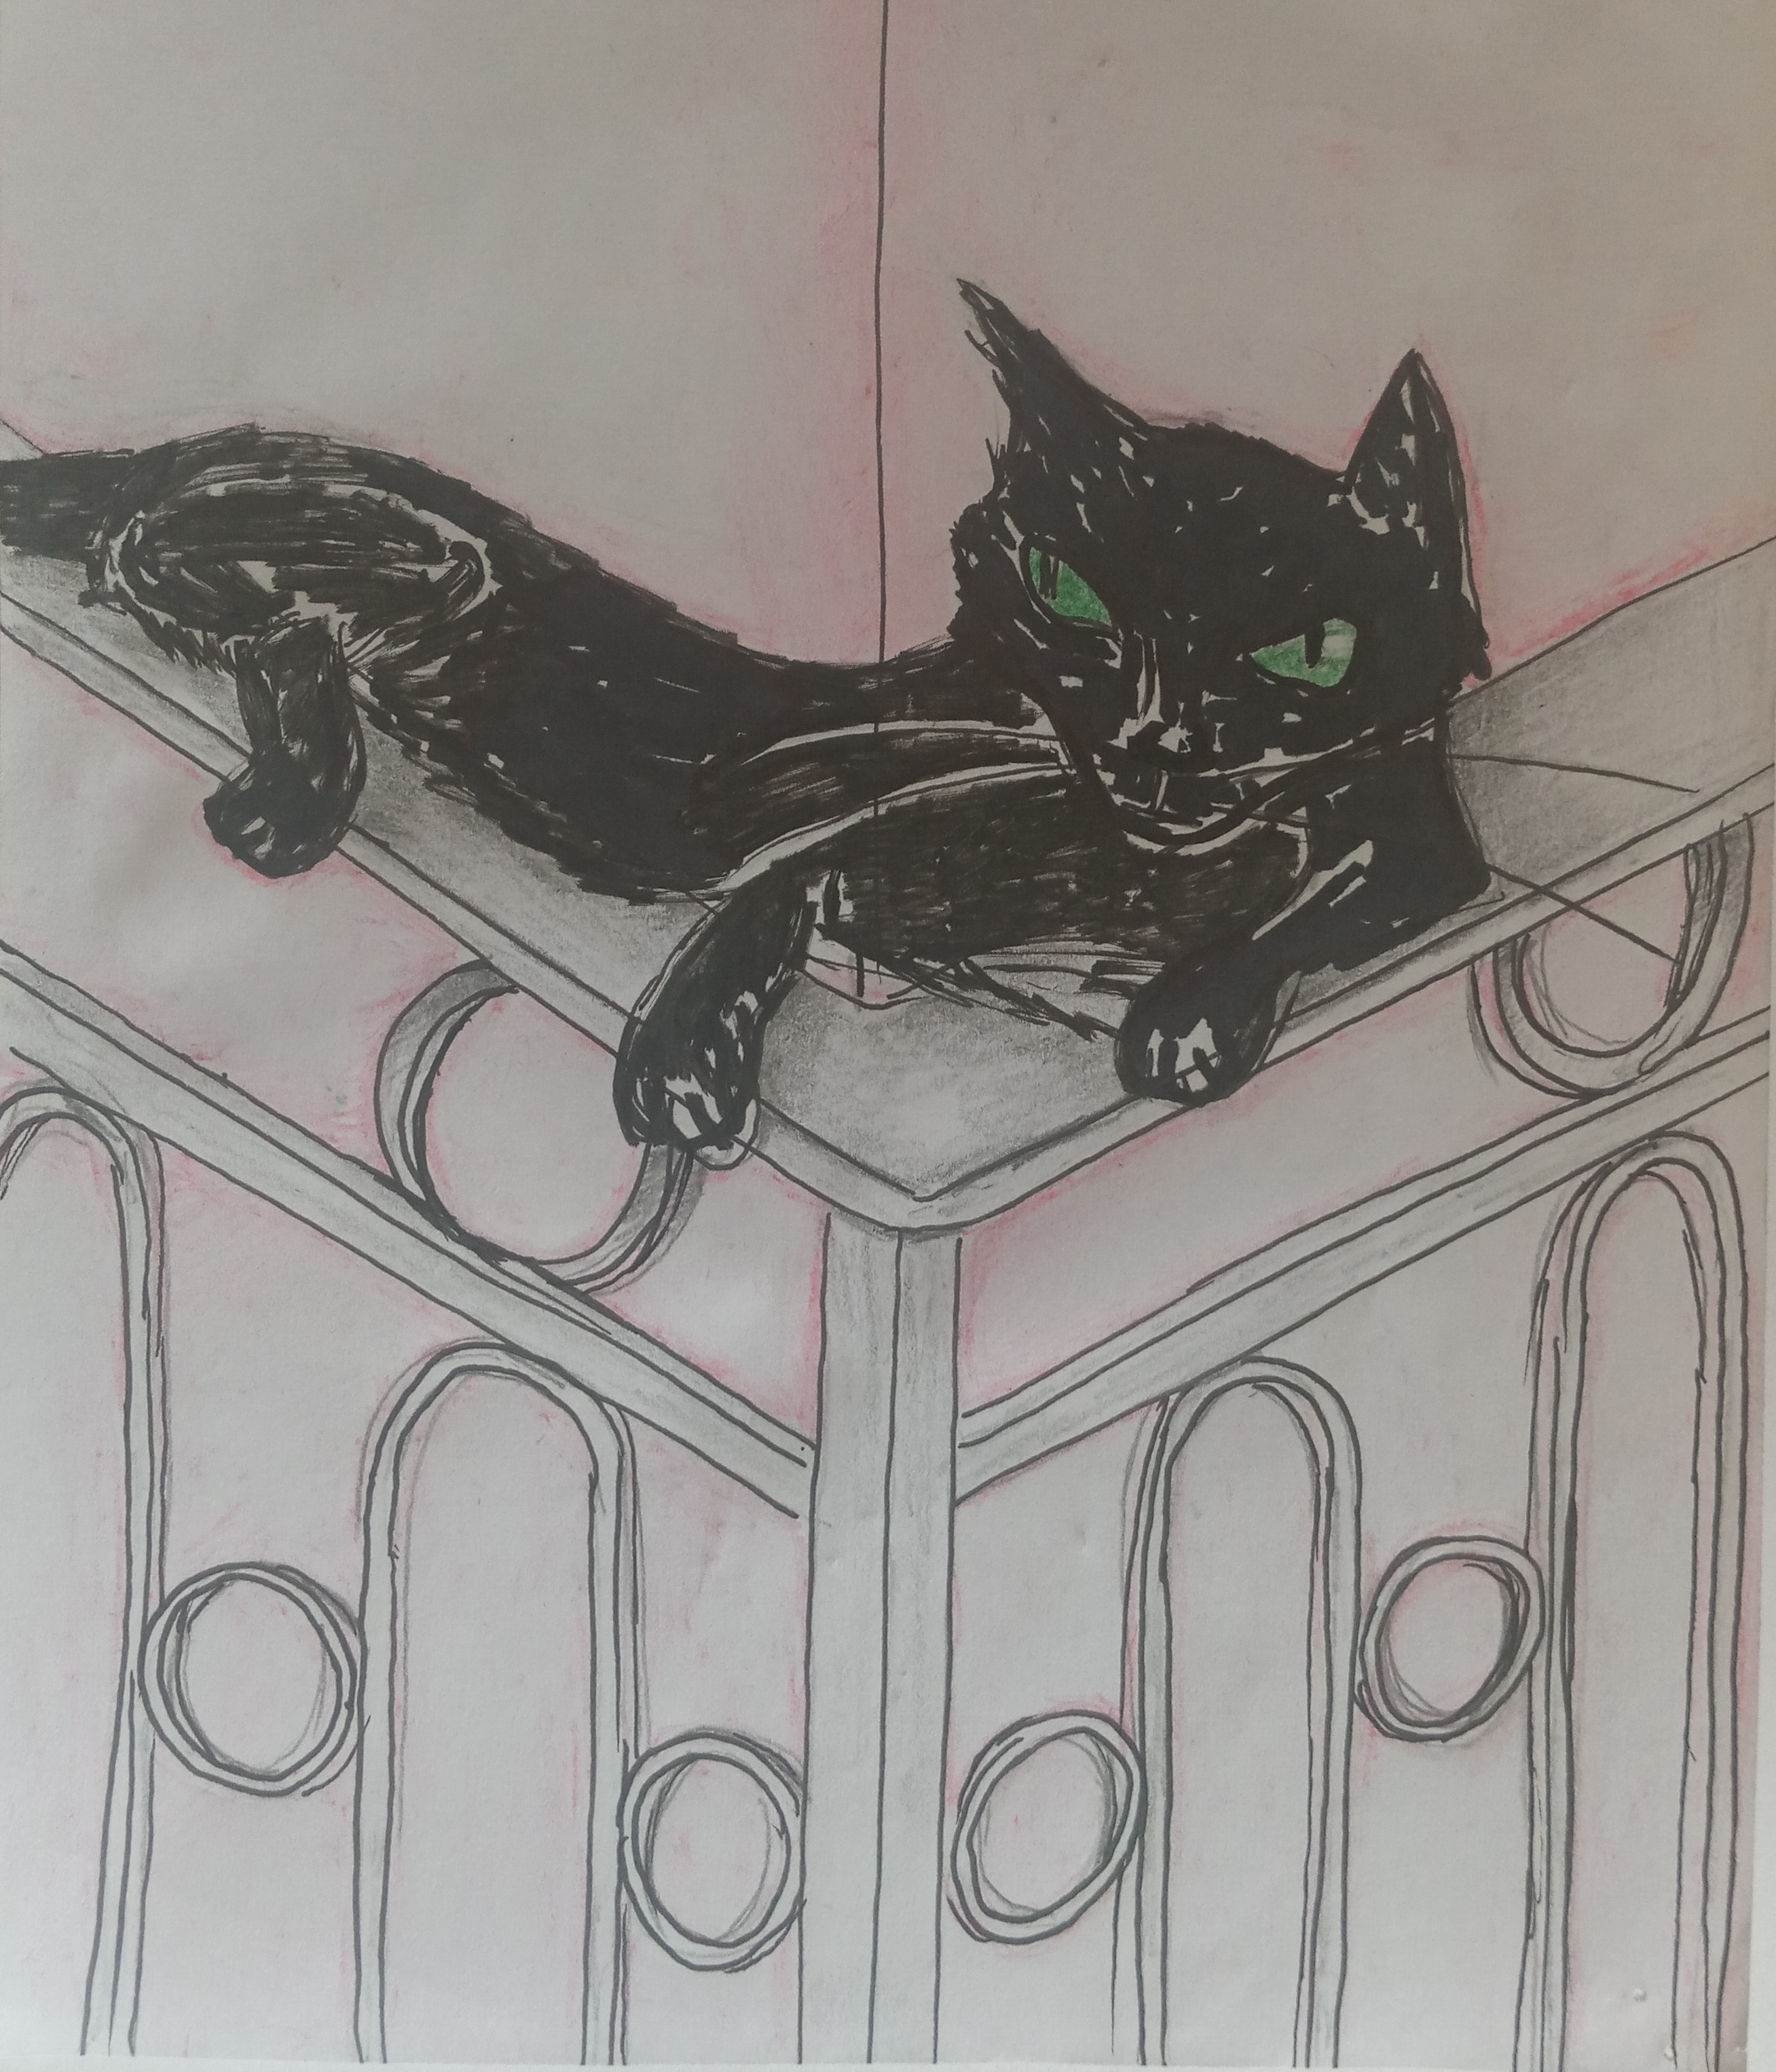
\includegraphics[width=.5\paperwidth,angle=0]{melissa1.png}};	
\end{tikzpicture}	
PERO, NINGUNO LO CONSEGUÍA, MELISSA AGUARDABA.

\newpage
\begin{tikzpicture}[remember picture, overlay]
	\node [inner sep=0pt, minimum width=\paperwidth, minimum height=\paperheight,opacity=.3,color=Apricot] at (current page.center) {\includegraphics[width=\paperwidth,height=\paperheight,angle=0]{paper25}};
\end{tikzpicture}
-ESO PORQUE YO NO ESTABA ALLÍ, DIJE CON ORGULLO, PRETENSIÓN	Y ALGO DE IMPRUDENCIA

-GATOS MÁS VALIENTES, FUERTES Y SALVAJES QUE VOS LO INTENTARON, QUERIDO OTTOKO, Y TODOS QUEDARON EN EL CAMINO, DIJO MORA CON FRIALDAD, Y PROSIGUIÓ:

LO HACÍAN POR LAS NOCHES, FORMANDO UN CORO DE MAULLIDOS, RONRONEOS Y RUGIDOS. LOS MUROS ALTOS IMPEDÍAN QUE LLEGARAN A MELISSA QUE DESCANSABA MIENTRAS ELLOS SE REPARTÍAN ARAÑAZOS, MORDIDAS, ZARPAZOS, EN FIN, UN CONCIERTO DE MALDADES FELINAS.

LOS GATOS MÁS FIEROS DEL BARRIO ACUDÍAN A LOS JARDINES DEL CASTILLO ABANDONADO. ENTRE LOS MÁS MALVADOS, SE DESTACABA PANCHO, UN MALINTENCIONADO DE COLOR BLANCO Y NEGRO, OREJAS RECORTADAS A MORDIDAS, MANDÍBULAS ENORMES, TORSO ANCHO Y 

\newpage
\begin{tikzpicture}[remember picture, overlay]
	\node [inner sep=0pt, minimum width=\paperwidth, minimum height=\paperheight,opacity=.3,color=Apricot] at (current page.center) {\includegraphics[width=\paperwidth,height=\paperheight,angle=0]{paper25}};
	\node [inner sep=0pt, minimum width=.9\paperwidth, minimum height=\paperheight,opacity=1,xshift=-.32\paperwidth,text width=.5\linewidth,yshift=-.05\paperheight] at (current page.center) {\includegraphics[width=.5\paperwidth,angle=0]{pancho1.png}};
	
	
\end{tikzpicture}
PREPOTENTE. NO TENÍA NINGÚN INTERÉS EN TREPAR, SINO MÁS BIEN EN EL DAÑINO DISFRUTE DE PELEAR. PERROS PEQUEÑOS Y HASTA LA GENTE LE TENÍA MIEDO AL FEROZ PANCHO. 
\begin{flushright}
	\begin{minipage}[r]{.56\textwidth}
		MUY POCAS  VECES HABÍA SIDO  DERROTADO Y LAS BATALLAS PODÍAN SUCEDERSE DURANTE HORAS.
		
		ESA ERA TODA LA COMPAÑÍA QUE TOLERABA LA SEÑORA BIGLIA. UNA RARA LEYENDA AFIRMABA QUE LA ANCIANA HABÍA NOMBRADO COMO HEREDERA A SU GATA Y A SU DESCENDENCIA. TODO ERA BASTANTE DELIRANTE ALREDEDOR DEL PALACIO DE LOS BICHOS.
	\end{minipage}
\end{flushright}



\newpage
\begin{tikzpicture}[remember picture, overlay]
	\node [inner sep=0pt, minimum width=\paperwidth, minimum height=\paperheight,opacity=.3,color=Apricot] at (current page.center) {\includegraphics[width=\paperwidth,height=\paperheight,angle=0]{paper22}};
	
\end{tikzpicture}
UNA TARDE DE 19.., UN ASTUTO GATO SE ASOMÓ POR LAS REJAS DE LA ENTRADA Y LUEGO SE SENTÓ SOBRE UNO DE LOS PILARES. TRANQUILO Y SONRIENTE SE PUSO A OBSERVAR Y PENSAR. ERA UN GATO DOMÉSTICO, NO FORMABA PARTE DE LAS BANDAS FELINAS QUE SE FORMABAN EN EL BARRIO. SU PELAJE ERA MUY CORTO,  DE COLOR  CLARO, Y POR ELLO SU ASPECTO TENÍA CIERTOS  TINTES ROSAS.  SU ASPECTO FLACO Y DESGARBADO NO ERA EL TÍPICO DE LOS GATOS PELEADORES DEL LUGAR.

NO LE INTERESABAN LAS RIÑAS, SE PRESENTABA POR LAS TARDES Y ALGUNAS NOCHES  SIN NUNCA PARTICIPAR. MIRABA LOS MOVIMIENTOS DE TODOS Y SE SENTABA EN EL MISMO PILAR COMO SI DISFRUTARA DE UN CONCIERTO DE MÚSICA CLÁSICA.  
LOS OTROS GATOS NO LE PRESTABAN NINGUNA ATENCIÓN, TAN SÓLO PARA BURLARSE DE SU ASPECTO. LE DECÍAN ´´EL PANTERA ROSA´´, COSA QUE SI BIEN NO ERA MUY AMABLE,  RESULTABA BASTANTE ACERTADA.



\newpage
\begin{tikzpicture}[remember picture, overlay]
	\node [inner sep=0pt, minimum width=\paperwidth, minimum height=\paperheight,opacity=.3,color=Apricot] at (current page.center) {\includegraphics[width=\paperwidth,height=\paperheight,angle=0]{paper25}};
	\node [inner sep=0pt, minimum width=.9\paperwidth, minimum height=\paperheight,opacity=1,xshift=-.32\paperwidth,text width=.5\linewidth,yshift=-.05\paperheight] at (current page.center) {\includegraphics[width=.5\paperwidth,angle=0]{boris1.png}};
\end{tikzpicture}
´´EL PANTERA ROSA´´, UN GATO TRANQUILO Y REFLEXIVO. PASARON LOS DÍAS SIN NOVEDAD, Y EL GATO ROSADO YA TENÍA UN PLAN PARA ALCANZAR LA TERRAZA, PUES CONFIABA EN SUS DOTES 	DE TREPADOR, 
\begin{flushright}
	\begin{minipage}[r]{.56\textwidth}
		QUE AYUDABAN SU DELGADEZ Y FLEXIBILIDAD. 
		
		HABÍA CALCULADO TODO EL TRAYECTO QUE IBA DESDE SU PILAR HASTA EL MURO QUE SOPORTABA EL BALCÓN DONDE MELISSA SOLÍA PASEAR. OTROS LO HABÍAN HECHO ANTES QUE ÉL, PERO SIN ESPERAR LO SUFICIENTE. 
	\end{minipage}	
\end{flushright}


\newpage
\begin{tikzpicture}[remember picture, overlay]
	\node [inner sep=0pt, minimum width=\paperwidth, minimum height=\paperheight,opacity=.3,color=Apricot] at (current page.center) {\includegraphics[width=\paperwidth,height=\paperheight,angle=0]{paper22}};
\end{tikzpicture}
PORQUE TODO INTENTO DE SUBIR ERA VISTO COMO UN DESAFÍO AL JEFE, A PANCHO, QUE NO PODÍA ESCALAR PERO SÍ PODÍA DAR TEMIBLES ZARPAZOS Y MORDEDURAS.
PARA QUEDAR BIEN CON EL, TODO UNA BANDA DE GATOS IMPEDÍA QUE NADIE PUDIESE TREPAR AL BALCÓN. LOS QUE LO INTENTABAN, LUEGO VOLVÍAN MUY MAGULLADOS A SUS CASAS.
PERO EL GATO ROSADO PASÓ DESAPERCIBIDO, NO LLAMÓ LA ATENCIÓN DE LA PANDILLA FELINA MÁS QUE PARA RECIBIR BURLAS. NINGUNO IMAGINÓ LO QUE TERMINÓ SUCEDIENDO.

SERÍAN LAS CINCO DE LA MAÑANA, LA MAYOR PARTE DE LOS GATOS YA DORMITABA CANSADOS DE TANTO MOLESTAR DURANTE HORAS A LOS VECINOS CON SUS MAULLIDOS. ALGUNOS VOLVÍAN A SUS CASAS CUANDO BORIS, EL GATO DE TINTES ROSAS, APARECIÓ DE UN BRINCO SOBRE SU PILAR DE TODOS LOS DÍAS. PANCHO DORMÍA PANZA ARRIBA SOBRE EL CÉSPED JUNTO A VARIOS DE SUS ADMIRADORES Y ADMIRADORAS. 
\newpage
\begin{tikzpicture}[remember picture, overlay]
	\node [inner sep=0pt, minimum width=\paperwidth, minimum height=\paperheight,opacity=.3,color=Apricot] at (current page.center) {\includegraphics[width=\paperwidth,height=\paperheight,angle=0]{paper22}};
\end{tikzpicture}
ERA UNA NOCHE DE LUNA LLENA, MUY APROPIADA PARA ANUNCIAR EVENTOS EXTRAORDINARIOS.
Y BORIS BAJÓ POR PRIMERA VEZ AL PATIO DE LAS PELEAS FELINAS, PERO PARA CRUZARLO VELOZ COMO UN RAYO. Y ALCANZÓ UNA GÁRGOLA DE ESAS DE FIGURAS ATERRADORAS Y SE SUBIÓ TRANQUILO SOBRE LA CABEZA. SE HIZO UN GRAN TUMULTO, CON TODO EL GATERÍO DESPERTANDO Y PROTESTANDO POR LA PROVOCACIÓN DEL ´´PANTERA ROSA´´. NO LO PODÍAN CREER!

EL BURLADO FLACUCHO, EL MENOS TEMIBLE DE TODOS LES HABÍA DADO UNA LECCIÓN DE ASTUCIA. PORQUE, A FIN DE CUENTAS, SER UN BRAVO FELINO TIENE QUE VER MÁS CON INGENIO QUE CON FUERZA. DESDE LA GÁRGOLA, TRIUNFANTE PERO MUY DISCRETO, ALCANZÓ UNA VENTANA APENAS ABIERTA QUE LO LLEVÓ A RECORRER EL SEGUNDO PISO DEL CASTILLO. 

\newpage
\begin{tikzpicture}[remember picture, overlay]
	\node [inner sep=0pt, minimum width=\paperwidth, minimum height=\paperheight,opacity=.3,color=Apricot] at (current page.center) {\includegraphics[width=\paperwidth,height=\paperheight,angle=0]{paper24}};
	\node [xscale=-1,inner sep=0pt,xshift=-.4\paperwidth,yshift=.41\paperheight] at (current page.center) {\includegraphics[width=.15\paperwidth,angle=0]{silueta1.png}};
\end{tikzpicture}
LA SALA POR DONDE INGRESÓ BORIS ERA MUY AMPLIA, 

LA LUZ DE LA LUNA ENTRABA POR LAS VENTANAS Y SUS REFLEJOS EN ESPEJOS PERMITÍAN QUE UN GATO PUDIERA FÁCILMENTE TODO.

TENÍA, COMO EL RESTO DE LAS HABITACIONES, UN ALTÍSIMO CIELO RASO. SE APRECIABAN MOLDURAS MUY DELICADAS, CON SUTILES MOTIVOS DE NOTAS MUSICALES ES CADA ESQUINA. EL PISO ERA DE MADERA, DE LARGAS PLACAS DE PINOTEA COMO SE PUEDEN VER EN LOS EDIFICIOS DE LA ÉPOCA. 
BAJO LOS PASOS DE UN HUMANO, PISO PODÍA RECHINA PERO NUNCA ANTE LAS DELICADAS ALMOHADILLAS DEL GATO ROSADO. MIRABA A UN LADO Y A OTRO, BUSCANDO PRIMERO LA PUERTA Y OTRAS VENTANAS QUE LE SIRVIERAN DE ESCAPE SI FUERA NECESARIO. 


\newpage
\begin{tikzpicture}[remember picture, overlay]
	\node [inner sep=0pt, minimum width=\paperwidth, minimum height=\paperheight,opacity=.3,color=Apricot] at (current page.center) {\includegraphics[width=\paperwidth,height=\paperheight,angle=0]{paper21}};
	\node [xscale=-1,inner sep=0pt,xshift=.4\paperwidth,yshift=.35\paperheight] at (current page.center) {\includegraphics[width=.15\paperwidth,angle=0]{silueta3.png}};
\end{tikzpicture}
RECIÉN ENTONCES SE PUSO A ADMIRAR LOS MUEBLES. 
\begin{flushright}
	\begin{minipage}[r]{.86\textwidth}
		ERA UN LUGAR MUY PARTICULAR. DISTINGUIÓ EN PRINCIPIO UN ENORME PIANO DE COLA CON UN PEQUEÑO TABURETE FRENTE A ÉL SOBRE EL QUE SALTÓ DE INMEDIATO.
		
	\end{minipage}
\end{flushright} 
EL PIANO TENÍA EL TECLADO DESCUBIERTO Y LA TAPA SUPERIOR SE
ENCONTRABA ABIERTA LEVEMENTE. BORIS CAMINÓ TAN DESPACIO SOBRE LAS TECLAS QUE NO LLEGÓ A OÍRSE NINGUNA NOTA. 

EN EL ATRIL HABÍAN DEJADO UNA PARTITURA ESCRITA A MANO, EN TINTA. EL FELINO AVENTURERO NADA SABÍA DE MÚSICA, PERO ADIVINÓ, POR LA CANTIDAD DE NOTAS DISTINTAS ESCRITAS, QUE NO DEBÍA SER FÁCIL EJECUTARLA. 

EL TÍTULO DECÍA ´´ESTELA FUGAZ´´ Y EL PAPEL TENÍA MANCHAS DE HABER SIDO UN POCO SALPICADO. EL MUY SENSIBLE GATITO IMAGINÓ QUE ALGUIEN HABÍA LLORADO FRENTE A LA PARTITURA Y SE ENTRISTECIÓ.


\newpage
\begin{tikzpicture}[remember picture, overlay]
	\node [inner sep=0pt, minimum width=\paperwidth, minimum height=\paperheight,opacity=.3,color=Apricot] at (current page.center) {\includegraphics[width=\paperwidth,height=\paperheight,angle=0]{paper24}};
\end{tikzpicture}
LEVANTÓ LUEGO SU VISTA PARA MIRAR ALREDEDOR Y RECONOCIÓ OTROS INSTRUMENTOS: HABÍA UN VIOLONCELO, DOS VIOLINES, DOS CLARINETES Y OTROS MÁS DE LOS QUE NO CONOCÍA EL NOMBRE. NO HABÍA INSTRUMENTOS DE METAL, ERAN DE CUERDA O VIENTOS DE MADERA. 

RECONOCIÓ TAMBIÉN DOS PERFUMES, UNO HUMANO Y OTRO FELINO, Y ESA INTRIGA LO LLEVÓ A ACERCARSE CON CUIDADO A LA PUERTA. NO ESTABA CERRADA Y DABA A UN PASILLO QUE ESTABA BIEN OSCURO. LA EMPUJÓ SUAVEMENTE CON SU PATA Y SE OYÓ UN CHIRRIDO.

ENSEGUIDA, ESCUCHÓ UNOS RUIDOS PESADOS COMO SI CAMINARAN SOBRE SU TECHO, SU CORAZÓN FELINO SE AGITÓ AUNQUE CONSERVÓ TODA SU SANGRE FRÍA. ESPERÓ UNOS MINUTOS ANTES DE VOLVER A ABRIR LO SUFICIENTE LA PUERTA COMO PARA PODER PASAR SUS BIGOTES. LA LUZ DE LA LUNA SE FILTRÓ UN POCO HACIA EL PASILLO Y PUDO VER APENAS 

\newpage
\begin{tikzpicture}[remember picture, overlay]
	\node [inner sep=0pt, minimum width=\paperwidth, minimum height=\paperheight,opacity=.3,color=Apricot] at (current page.center) {\includegraphics[width=\paperwidth,height=\paperheight,angle=0]{paper17}};
	\node [xscale=1,inner sep=0pt,xshift=.4\paperwidth,yshift=.4\paperheight] at (current page.center) {\includegraphics[width=.15\paperwidth,angle=0]{silueta4.png}};	
\end{tikzpicture}	
LO QUE AGUARDABA.
ANTES DE SALIR DE LA SALA 
DE 

MÚSICA, BORIS, ATENDIENDO A SUS BIGOTES, A LA LUZ DE LA LUNA, RECORDÓ UNA CANCIÓN DE NIÑEZ QUE SIEMPRE LE HIZO REÍR. DECÍA:
\begin{center}
	\begin{minipage}{.5\textwidth}
		´´EL SOL SE DEJÓ CRECER, CRECER LOS BIGOTES,
		
		LA LUNA CUANDO LO VÍO,
		
		LE DIJO ¡QUE BIGOTÓMATES!´´
	\end{minipage}
\end{center}	
JIJIJI, ¡QUE DULCE Y LINDA LA NENA  QUE LE CANTABA ASÍ HACE TANTOS AÑOS!

SE ESCURRIÓ POR FIN AL PASILLO Y NOTÓ QUE EL PISO ERA MÁS FRÍO ALLÍ. PUDO VER QUE HABÍA TRES OTRAS SALAS PERO TUVO MÁS CURIOSIDAD EN IR HACIA LA ESCALERA EN ESPIRAL AL FONDO DEL PASILLO.
